% !TEX program = xelatex

\documentclass[12pt,a4paper]{article}
\usepackage[UTF8]{ctex}
\usepackage{float}
\usepackage{amsmath}
\usepackage{enumerate}
\usepackage{booktabs}
\usepackage{graphicx}
\usepackage{longtable}
\usepackage{subfigure}

\usepackage{url}

% for plotting 
\usepackage{caption}
\usepackage{pgfplots}

% for pseudo code 
\usepackage{algorithm}
\usepackage[noend]{algpseudocode}

% for reference 
\usepackage{hyperref}
\usepackage{cleveref}

% for code 
\usepackage{listings}
\usepackage{xcolor}
\usepackage{fontspec}

\newfontfamily\consolas{Consolas}
\definecolor{darkgreen}{rgb}{0,0.6,0}

% Microsoft Word A4 paper default layout 
\usepackage[a4paper, left=3.18cm, right=3.18cm, top=2.54cm, bottom=2.54cm]{geometry}

\captionsetup[figure]{labelfont={bf}, name={Figure}}
\captionsetup[table]{labelfont={bf}, name={Table}}

\title{信号处理原理实验报告}
\author{2017011620 计73 李家昊}
\date{\today}

\begin{document}

\maketitle

\section{实验1}

本实验中实现了Goertzel算法识别DTMF音频信号,并在速度和精度上与FFT做了对比。

\subsection{标准音频测试}

在网上下载了按键0-9的DTMF音频,分别用FFT和Goertzel算法识别,测试结果如\Cref{tab:standard}所示。

\begin{longtable}[]{c|c|cccc}
    \toprule
    Key & Length & Goertzel Result & Goertzel Time (s) & FFT Result & FFT Time (s)\tabularnewline
    \midrule
    \endhead
    0 & 4687 & 0 & 0.001912 & 0 & 0.002677\tabularnewline
    1 & 4049 & 1 & 0.001160 & 1 & 0.002206\tabularnewline
    2 & 3731 & 2 & 0.001244 & 2 & 0.002253\tabularnewline
    3 & 5254 & 3 & 0.001684 & 3 & 0.002409\tabularnewline
    4 & 5326 & 4 & 0.002075 & 4 & 0.002727\tabularnewline
    5 & 4523 & 5 & 0.001485 & 5 & 0.002248\tabularnewline
    6 & 5613 & 6 & 0.001662 & 6 & 0.002197\tabularnewline
    7 & 5071 & 7 & 0.001887 & 7 & 0.002594\tabularnewline
    8 & 4918 & 8 & 0.001498 & 8 & 0.002282\tabularnewline
    9 & 4658 & 9 & 0.001441 & 9 & 0.002234\tabularnewline
    \bottomrule
    \caption{Goertzel和FFT算法的标准单按键音频测试结果}
    \label{tab:standard}
\end{longtable}

可以看出,在精度上,两种算法的预测结果都非常准确,在速度上,Goertzel比FFT更快一些,原因是其计算量更小,且序列长度并不大。

\subsection{实际音频测试}

接下来用手机拨打我的电话13380831033,并用笔记本电脑将按键音频录制下来,其中伴随少量环境噪声,原始时域信号如\Cref{fig:phone_number}所示。

\begin{figure}[htbp]
    \centering
    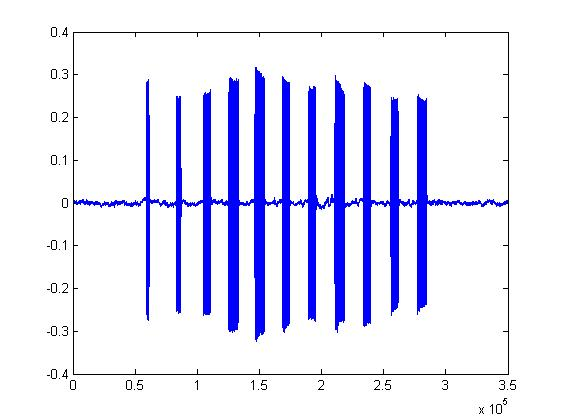
\includegraphics[width=\textwidth]{fig/phone_number.jpg}
    \caption{实际音频的时域信号}
    \label{fig:phone_number}
\end{figure}

从音频的第57000个采样点处开始,每22000个采样点为一个按键,共分成11个按键,取每个按键的前5000个采样点,分别采用Goertzel和FFT算法测试,结果如\Cref{tab:practical}所示。

\begin{longtable}[]{c|cccc}
    \toprule
    Key & Goertzel Result & Goertzel Time (s) & FFT Result & FFT
    Time (s)\tabularnewline
    \midrule
    \endhead
    13380831033 & 13380831033 & 0.010394 & 13380831033 &
    0.025543\tabularnewline
    \bottomrule
    \caption{Goertzel和FFT算法的实际多按键音频测试结果}
    \label{tab:practical}
\end{longtable}

可以看出,在实际情况下,两种算法都给出了精确的结果,但在速度上Goertzel仍然比FFT更快。

\section{实验2}

本实验中实现了四种卷积算法,为评测它们的性能,令序列总长度$L$从2递增到5000,令序列$x$的长度$L_x$在$[1, L-1]$中随机产生,序列$y$的长度为$L_y = L - L_x$,序列$x,y$的内容均随机生成,用四种算法分别计算$x*y$,统计所用的时间,测试结果如\Cref{fig:conv}所示。可以看出,直接按公式计算的效率明显低于其他三种算法,其他三种算法性能相当,FFT的速度略低于Overlap-Add和Overlap-Save,因为这两种算法在$L_x$和$L_y$相差较大时具有不错的加速效果。

\begin{figure}[htbp]
    \centering
    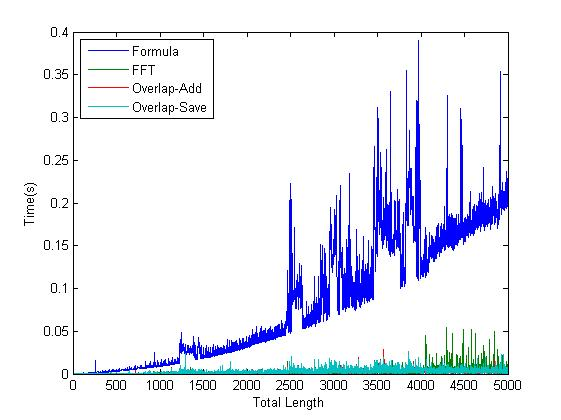
\includegraphics[width=\textwidth]{fig/conv.jpg}
    \caption{四种算法的运行时间随序列总长度的变化曲线图}
    \label{fig:conv}
\end{figure}

\section{实验3}

本实验中模拟了频分复用(FDM)的编码和解码过程。设有$n$个长度为$L$的音频,如图\Cref{fig:original}所示,在调试过程中,将每个音频上采样$n$倍,如图\Cref{fig:upsampled}所示,然后通过FFT得到频域信号,通过滤波器互不重叠地提取每个音频频谱中的一个周期,将这些频谱信号叠加起来,就得到了调制信号,如图\Cref{fig:modulated}所示。在解调过程中,用滤波器将对应频段的调制信号提取出来,再进行IFFT即可得到时域信号,如图\Cref{fig:decoded}所示。

\begin{figure}
    \centering
    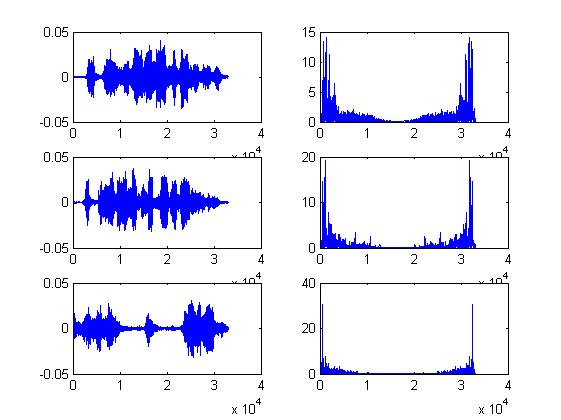
\includegraphics[width=\textwidth]{fig/original.jpg}
    \caption{原始的时域信号(左)及频域信号(右)}
    \label{fig:original}
\end{figure}

\begin{figure}
    \centering
    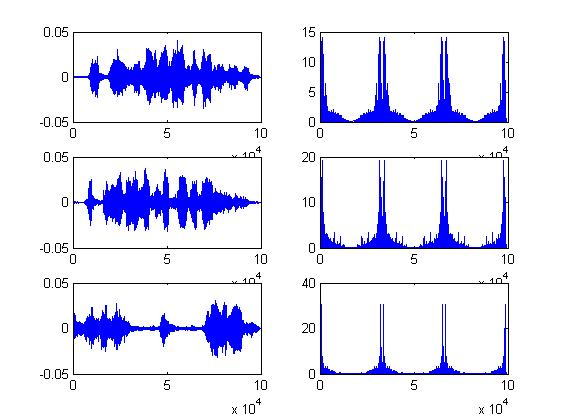
\includegraphics[width=\textwidth]{fig/upsampled.jpg}
    \caption{上采样后的时域信号(左)及频域信号(右)}
    \label{fig:upsampled}
\end{figure}

\begin{figure}
    \centering
    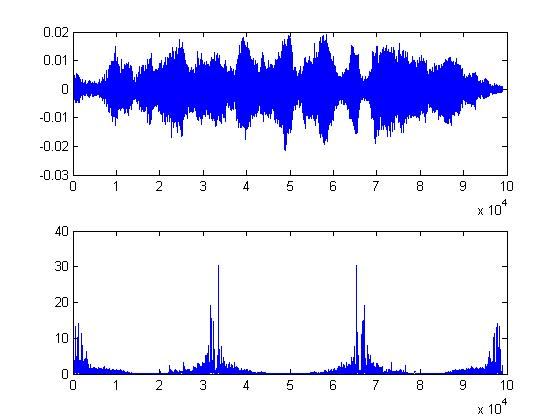
\includegraphics[width=\textwidth]{fig/modulated.jpg}
    \caption{调制后得到的时域信号(上)及频域信号(下)}
    \label{fig:modulated}
\end{figure}

\begin{figure}
    \centering
    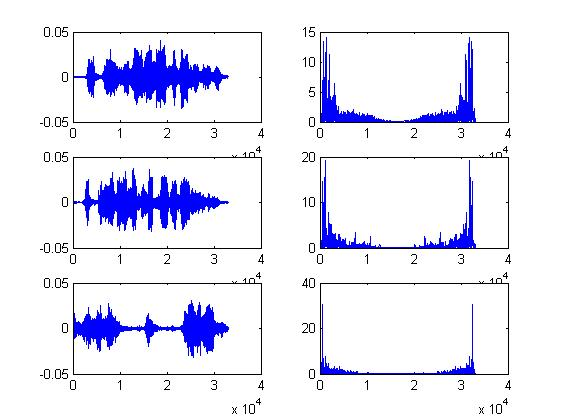
\includegraphics[width=\textwidth]{fig/decoded.jpg}
    \caption{解调后得到的时域信号(左)及频域信号(右)}
    \label{fig:decoded}
\end{figure}

\end{document}